\documentclass{standalone}
\usepackage{tikz}
\usepackage{ctex,siunitx}
\usepackage{tkz-euclide}
\usepackage{amsmath}
\usetikzlibrary{patterns, calc}
\usetikzlibrary {decorations.pathmorphing, decorations.pathreplacing, decorations.shapes,}
\begin{document}
\small
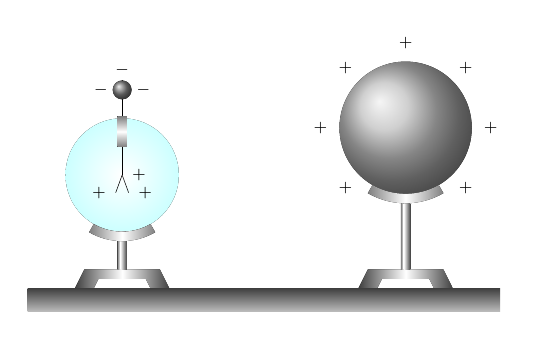
\begin{tikzpicture}[>=latex,scale=1.2]
  % \useasboundingbox(-1,-2)rectangle(8,6);
  \fill[inner color=white, outer color=cyan!20](0,0)circle(0.6);
  \fill[left color=darkgray,right color=darkgray, middle color=white](-0.5,-1.2)--++(0.2,0)--++(0.05,0.1)--++(0.5,0)--++(0.05,-0.1)--++(0.2,0)--++(-0.1,0.2)--++(-0.8,0)--cycle;
  \fill[left color=gray,right color=white](-0.05,-0.6)rectangle(-0.02,-1.0);
  \fill[left color=white,right color=darkgray](-0.02,-0.6)rectangle(0.05,-1.0);
  \fill[left color=gray,right color=gray, middle color=white](300:0.6)arc(300:240:0.6)--(240:0.7)arc(240:300:0.7)--cycle;
  \fill[top color=gray,bottom color=gray,middle color=white](-0.05,0.3)rectangle(0.05,0.62);
  \draw(0,0.62)--(0,1.0);
  \draw(0,0.3)--(0,0)node[right]{\tiny$+$};
  \draw[very thin](0,0)--(250:0.2)node[left]{\tiny$+$}(0,0)--(290:0.2)node[right]{\tiny$+$};
  \fill[ball color=gray](0,0.9)circle(0.1)node[above=0.5mm]{\tiny$-$};
  \node at (0,0.9)[left=0.5mm]{\tiny$-$};
  \node at (0,0.9)[right=0.5mm]{\tiny$-$};
  \begin{scope}[xshift=3cm,yshift=5mm]
    \fill[ball color=lightgray](0,0)circle(0.7);
  \fill[left color=darkgray,right color=darkgray, middle color=white](-0.5,-1.7)--++(0.2,0)--++(0.05,0.1)--++(0.5,0)--++(0.05,-0.1)--++(0.2,0)--++(-0.1,0.2)--++(-0.8,0)--cycle;
  \fill[left color=gray,right color=white](-0.05,-0.8)rectangle(-0.02,-1.5);
  \fill[left color=white,right color=darkgray](-0.02,-0.8)rectangle(0.05,-1.5);
  \fill[left color=gray,right color=gray, middle color=white](300:0.8)arc(300:240:0.8)--(240:0.7)arc(240:300:0.7)--cycle;
  \foreach \x in {-45,0,...,225}
  {
    \node at (\x:0.9) {\tiny$+$};
  }
  \end{scope}
  \fill[top color=darkgray,bottom color=lightgray](-1,-1.2)rectangle(4,-1.45);
\end{tikzpicture}
\end{document}